%File: formatting-instruction.tex
\documentclass[letterpaper]{article}
\usepackage{aaai}
\usepackage{times}
\usepackage{helvet}
\usepackage{courier}
\usepackage{hyperref}
\usepackage[round]{natbib}
\usepackage{graphicx}

\nocopyright
\frenchspacing
\pdfinfo{
/Title (Classification of Tweets by Company)
/Author (Curtis Ullerich, Daniel Stiner, Brandon Maxwell)}
\setcounter{secnumdepth}{0}  
\begin{document}

\title{Tweet Classification: Filtering \\ of Twitter for Company-relevant Tweets}
\author{
Curtis Ullerich, Daniel Stiner, Brandon Maxwell\\
Department of Computer Science and Engineering\\
Iowa State University
Ames, Iowa, USA\\
\{curtisu,stiner,bmaxwell\}@iastate.edu\\
}
\maketitle
\begin{abstract}
\begin{quote}
Twitter is a popular source for data mining due to its massive scale and inclusivity of current trends.
It is also a veritable goldmine of useful data for businesses seeking to discover public opinion about themselves or their products.
Using machine learning techniques, we analyze the accuracy of classifying whether tweets directly mention a particular company or mearly contain keywords related to the company.
%Tweets present interesting classification challenges due to their irregular formatting and relatively small number of features.
%Classification purely by keyword filtering often suffers from a
%high accuracy and low recall, or low accuracy and high recall. % Q: Daniel - What does recall mean in this context? Also, list low accuracy first I think.
We aim to survey a variety of text processing steps combined with a Naive Bayes classifier, focusing on the effects of different tokenizations.
Our dataset consists of approximately 2,000 tweets of which 64\% directly mention the company Apple, Inc or one of its products. The other 36\% do not, but still contain keywords related to the company.
Preliminary results have shown significant increases in accuracy % TODO insert actual numbers
by using domain-specific tokenizers, while surprisingly showing decreases in classification accuracy for other standard preprocessing methods such as n-grams.%maybe?
\end{quote}
\end{abstract}

\section{Introduction}
Tweets are used as a source of data mining for applications ranging from predicting future stock price changes based on user sentiment (\citeauthor{Ruiz}) and identifying characteristics of Twitter users (\citeauthor{conf/icwsm/PennacchiottiP11}) to tracking political protests and uncovering scams (\citeauthor{ICWSM101540}).
In many cases, the problem of determining which tweets are relevant for a particular application is prerequisite to meaningful results. Use of hashtags and username references on Twitter through syntax conventions (prepending with \# and @, respectively) can be used to select a subset of the tweets about a particular topic. 

\begin{table}[h]
\centering
\begin{tabular}{|l|}
	\hline
\textbf{@Apple} please make a squid \textbf{\#emoji} so I can put \\
one next to \textbf{@squidneyy22}'s name\\ \hline
Maybe \textbf{\#Apple} will release \textbf{\#iTunes11} \\
tomorrow. Maybe? \\ \hline
\end{tabular}
\caption{Hashtags and username references (note that Apple Inc. does not own the handle @Apple, though it is commonly used this way)}
\label{tab:myfirsttable}
\end{table}

In some domains, filtering tweets based solely on keywords may be appropriate, but disambiguation remains an interest natural language processing problem in many cases, particularly when the topic in question is a commonplace (and thus ambiguous) word, such as `apple,' `blackberry,' `android,' or `adobe' (\citeauthor{journals/ijcsa/YervaMA12}). 

Additionally, tweets contain a high rate of errors in grammar, spelling, and punctuation. These features are present alongside myriad augmentations of the English language due to internet trends and culture, as well as the desire of packing more information into Twitter's 140-character message limit (\citeauthor{Laboreiro:2010:TMM:1871840.1871853}). Preprocessing is necessary to avoid discarding or misinterpreting these features as noise or part of other tokens during tokenization.

\begin{table}[h]
\centering
\begin{tabular}{|l|}
	\hline
\textbf{Nvm} i'll buy you an ipad \textbf{\^-\^} \\ \hline
\#Apple fires `maps' project manager \textbf{loooool} big \\
 news story here in San Francisco! Go figure. \textbf{:-)} \\ \hline
Think I might have a \textbf{gf}! \textbf{O\_o} oh \\
lord\textbf{..} Lets see how this goes. \\ \hline
\end{tabular}
\caption{Examples of emoticons and common abbreviations found on Twitter}
\label{tab:myfirsttable}
\end{table}

We present a system to disambiguate tweets about the company Apple using a Naive Bayes model, increasing its baseline accuracy by 8\% through use of specialized, Twitter-aware tokenization.

\section{Related Work}
DUALIST is a system that extends Mallet, our machine learning API of choice, by user-interactive feedback during training (\citeauthor{Settles:2011:CLF:2145432.2145588}). Included in his implementation was a preprocessing step that performed some simple Twitter-specific feature extraction and tokenization. Part of the Sentiment Analysis Symposium focuses on Twitter-aware tokenization of tweets for sentiment analysis, demonstrating that it provides consistent improvement over whitespace- and Treebank-based tokenization \cite{potts2011}. A good deal of research has been done into sentiment classification of tweets, which requires very similar text processing and tokenization \cite{Pak10}. Laboreiro et al focus on the problem of tokenizing, using support vector machines (SVM) to improve upon the accuracy of rule-based tokenization, succeeded in improving from 85\% to 96\% token accuracy (\citeauthor{Laboreiro:2010:TMM:1871840.1871853}). Yerva et al construct classifiers to disambiguate tweets containing company-related keywords, primarily using profiles containing company background knowledge (\citeauthor{journals/ijcsa/YervaMA12}). Sriram et al presented a system that uses features extracted from the tweet author's profile and the tweet text to classify tweets into the categories of News, Events, Opinions, Deals, and Private Messages (\citeauthor{Sriram:2010:STC:1835449.1835643}).

\section{Method}
\subsection{Corpus creation}
By accessing the Twitter `Firehose' stream through their public API, we harvested 100,000 tweets using broad keyword filters with the goal of collecting a superset of relevant tweets. This provides us a smaller set of features in the overall corpus, with a much higher prior confidence that each individual tweet is of interest. The keywords used for the company of choice during this round of testing, Apple, were collected manually from information on the company's website and the Wikipedia page about Apple:\\

[INSERT LIST OF KEYWORDS]...\\
"apple", "itunes", "ipad", "ipod", "mac", "ios", "iphone", "AAPL", "cupertino", "safari", "ilife", "iwork", "garageband", "ibook", "powerbook", "itouch", "app store", "macworld", "facetime", "icloud", "mobileme", "siri", "imovie", "iphoto", "quicktime", "logic pro", "think different" \\

This set of keywords clearly allows a large number of false positives:

\begin{table}[h]
\centering
\begin{tabular}{|l|}
	\hline
	nice fish and chip.. good pie apple :-) \\ http://t.co/KVDN5r5l \\ \hline
	20 chicken nuggets, chips, big mac, and a \\ vanilla milkshake LIFE IS GOOD \\ \hline
	1 more day whoop plus safari ride yay \\ \hline
	Ashley staples an apple.  `AHHHH!!!! \\ Apple juice in my eye!' \\ \hline
	I ain't seen uncle Mac in a while \\
	\hline
\end{tabular}
\caption{Examples of false positive tweets}
\label{tab:myfirsttable}
\end{table}


We define a tweet to be `about' Apple if the tweet mentions the company (via direct reference or stock symbol), one of its products, or a service it offers. We make the assumption that spam will be filtered from the testing set. This could be done via an existing Naive Bayes classifier %[INSERT REFERENCE FOR TWEET SPAM FILTERING]
, but we simply did not include instances of spam in our corpus during the manual labeling process. We collected our tweets over the course of twelve hours. On Twitter, a single message posted is often reposted, or `re-tweeted,' many more times in a very short timespan. Because of the small timespan of our data collection, a large number of retweets (effectively duplicates) appeared in the dataset. We filtered these duplicates out of the dataset as well to prevent over-fitting in our model. After filtering, our original set of 100,000 tweets was reduced to 50,000. A representative sample of non-spam, non-duplicate tweets has a composition of 64\% topical instances and 36\% false positives.

\begin{table}[h]
\centering
\begin{tabular}{|l|}
	\hline
	I've collected 10,650 gold coins! \\ http://t.co/H0V0O6yP \#ipad, \#ipadgames, \#gameinsight\\
	\hline
\end{tabular}
\caption{A computer-posted spam tweet}
\end{table}

\begin{table}[h]
\centering
\begin{tabular}{|l|}
	\hline
	RT @PHILerNotebook: Trying to fix my Mac. \\ This gray loading bar takes 10 minutes to start up. \\ Grr. Shall take it to an \_Apple\_ \_store\_ soon! \\
	\hline
\end{tabular}
\caption{A retweet, signified by `RT'}
\end{table}

We hand labeled 2000 tweets for use in training and testing, including only English-language tweets in our training set. \\
Data sets and scripts used for processing text data are available on the project website. (http://tweets.curtisullerich.com/)\\

\subsection{Preprocessing Pipeline}

We do all machine learning with the Mallet library developed by the University of Massachusetts \cite{McCallumMALLET}. Mallet includes abstractions for a data processing pipeline, during which we use both existing and custom processing `Pipes' to transform the data, beginning in our case with raw tweet text and ending in Mallet's internal FeatureVector format. We built and tested several Pipes to analyze the effect of different filters and processes on the accuracy of classification. Not every Pipe proved to increase accuracy--some decreased it, as presented in the results. We present the descriptions of and motivations for these Pipes here.

\subsubsection{Feature-space Enrichment} ~\\
\textit{Stopword removal}: We used Mallet's TokenSequenceRemoveStopwords Pipe to remove 500 of the most common words in the English language from each tweet. We remove these words because of the high likelihood of many tweets containing these words, without contributing significant discriminatory features to the tweets. %TODO [REFERENCE NLP PAPER ABOUT STOPWORD REMOVAL]
\\
~\\
\textit{Bigrams}: Using n-grams is a common method of increasing the number of features present in short text%[FIND CITATION]
. Often, this is enough to increase accuracy significantly%CITATION
. As discussed in the tokenization section below, we used selective bigramming, which yielded increases in accuracy in almost all test cases.\\
~\\
\textit{HTML corrections}: When accessing tweets through Twitter's public API, the native JSON format includes HTML-encoded entities that can add confusing features to the tweets if not un-escaped. For instance, angle brackets are replaced with \&lt; and \&gt; (less-than and greater-than), causing emoticons, for instance, to no longer be parseable. The emoticon `\textgreater.\textless', for instance, would be `\&gt;.\&lt;'. Necessarily, this Pipe un-escapes all such entities, making them easier to parse.\\
~\\
\textit{URL replacement}: In our dataset, 60\% of the 100,000 tweets we collected contained a link. As the vast majority of these are unique, and shortened using a URL shortener, often Twitter's own t.co. Links, then, lose any features that may have been parsed from the URL, which often contains a domain name or title that may be useful in discriminating especially ambiguous links. Consider, for instance, the tweet `hmmm http://t.co/39D8I3qM' which leaves a parser completely unaware of the true content of the tweet. Following this URL leads to `http://www.redmondpie.com/iphone-5-vs-iphone-4s-should-you-upgrade/', which is clearly related to Apple. This pipe replaces the link itself in the tweet with the title of the destination web page: `iPhone 5 vs iPhone 4S: Should You Upgrade? | Redmond Pie.' In cases where the title is empty, we instead replace the shortened link with the resolved URL, which is `http://www.redmondpie.com/iphone-5-vs-iphone-4s-should-you-upgrade' in this case. In many cases like this, there is not other way to distinguish the content of a tweet. From our dataset of 100,000 tweets, 102 tweets contained \textit{only} a link, while 608 tweets contained only a link and fewer than 20 other characters. While this is a fairly small portion of the overall dataset for training purposes, it can be crucial in making decision on novel test instances. Pak and Paroubek also noted the need to handle URLs in tweets, however, rather than adding any new text, they chose to remove the link entirely  (\citeauthor{PAK10.385}).
~\\
\textit{Spell checking}: Twitter's user-generated content contains a large volume of misspelled words (\citeauthor{Laboreiro:2010:TMM:1871840.1871853}). Using a spell-checking library, we wrote a Pipe to replace unrecognized words (misspelled words) with their corrections if the confidence for correction was above a certain threshold. Our intention was to reduce the noise in the feature set by eliminating common misspellings.
~\\
\subsubsection{Disambiguation}
~\\
\textit{Stemming}: Stemming is the process of reducing words to their `stem,' in order to group different forms of the same word into a single feature. While this stem does not necessarily have to be the root of the word, it should satisfy the property that related words have the same stem. For instance, the stem of the related words `argue,' `argued,' and `arguing' all have the stem of `argu,' even though argu is not the true linguistic stem, or a real word. We used the standard Porter stemmer to implement this (\citeauthor{porter_1980}).
In some cases, stemming proved to increase our accuracy.
\\

\begin{figure*}[t!]
\centering
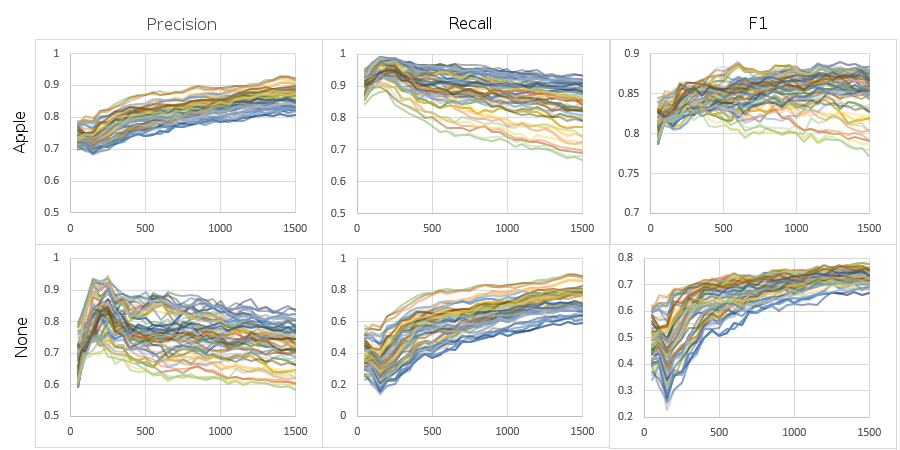
\includegraphics[height=7cm]{img/all-with-headings}
\caption{Metrics for all Pipeline combinations, training set sizes 50 through 1500 instances}
\label{fig:chart_all}
\end{figure*}

\subsubsection{Tokenization}
~\\
Tokens are atomic symbols in text that we use as features in training a classifier (\citeauthor{Laboreiro:2010:TMM:1871840.1871853}). Twitter data, and user-generated web content in general, provides unique challenges to an automatic tokenization system due to the high level of noise in the feature set. Tweets are limited to 140 characters, which limits the total number of features possible. Some of the many natural language processing dilemmas present in tweets include excessive and irregular punctuation, frequent misspellings, emoticons, URLs, and hashtags, as discussed in the introduction.\\

\begin{table}[h]
\centering
\begin{tabular}{|l|}
	\hline
	Cool ranch , 4 berry sundae , apple juice \textbf{\#yessuh} \\ 
	\textbf{\#latenight \#snack} http://t.co/ttc3vujp \\ \hline
	I just poured apple juice on my cereal\textbf{..} Gah. \textbf{\#SoTired} \\ \hline
	I hate Siri\textbf{.. -\_\_\_-} \\
	\hline
\end{tabular}
\caption{Examples of difficult tokenizations}
\label{tab:tokenization_examples}
\end{table}

Searching for emoticons in the tweet `Now on my iphone ?? http://t.co/Rqr1RL2R' will extract `:/' as an emoticon, effectively breaking up the URL token. Additionally, users often include emoticons or links after text with no delimiting whitespace, such as `I listen to my iPod every day and it's just broke \textbf{omg:(!!}.' We approach this problem using a layered token extraction system. Our goal is that any token pattern which may contain false positives of other tokens (e.g. emoticons inside URLS) is extracted before any potential interior false positive tokens. Extracting tokens using our layered approach eliminates many problems introduced by Twitter's unique feature space. Note that compiling an exhaustive list of all emoticon combinations is difficult, if not impossible, because the landscape of emoticons is very diverse and changes over time (\citeauthor{Laboreiro:2010:TMM:1871840.1871853}). Instead, we focus on capturing a `large enough' set of emoticons by extracting a large number of the most common ones. \\

After tokenizing these special features in order (URLs, emoticons, usernames, and hashtags) we are left with a fragmented tweet containing myriad punctuation, capitalization, and creative spellings. As done by \citet{potts2011} we normalize the length of all letter sequences greater than two, as in English these are invariably due to user-added emphasis, and condensing the larger set of tokens focuses the feature set. In the following tweet, for instance, `loooool' is normalized to `loool'.
\begin{quote}
\#news can't wait for my signed \#OoRITE2OutNow it's emotional here right now \textbf{loooool} \#OoRITE2OutNow https://t.co/r4n4cn6C 
\end{quote}

Note that such repetitions are often valid in URLs and some emoticons. Normalizing them prior to this step would make URLs invalid if using our link replacement Pipe.

As presented in our results, because of irregular capitalization, two tokens likely to be semantically identical with respect to company classification may be represented in multiple cases. {Nooo, NOOO, nooo, NoOo} is a prime example. To alleviate this, we attempt three different approaches. In the first, we simply lowercase all remaining tokens (note that many URLs become invalid after modifying case). In the second, we lowercase any text that is not in all caps. This serves to retain acronyms and any text specifically placed in all caps, while combining words capitalized because of sentence boundaries with their lowercase appearances, for instance. In the third approach, we change all remaining tokens to lowercase, except for leaving the case of all strings containing `apple' (case insensitive) alone. We made this decision based on the semantic difference between the capitalization of Apple the company and apple the fruit, which is a very significant feature in our dataset. While correct capitalization is naturally not always present for this token, this is one case where capitalization serves to disambiguate. In our dataset, `Apple' appeared 11784 times in 10500 tweets, `apple' appeared 4765 times in 4508 tweets, and other case-variations appeared 292 times in 237 tweets (all but one of which was `APPLE'). This same principle can be generalized to a larger set of keywords and applied to other companies in a similar fashion. \\

Optionally, our tokenizer will remove the token `RT' from all tweets. 3986 tweets in our dataset contain this token, signifying a retweet. Not knowing whether this feature added discriminatory power to our classifier, we toggled its inclusion during testing and found that removing it did lead to a slight increase in accuracy on our tests.\\

Any tokens remaining at this point during tokenization are very likely to be words in phrases. In order to focus the feature set, we split by whitespace and remove any non-word characters other than percent and dollar signs, stripping punctuation, quotation marks, parentheses, etc. \\

We chose to apply bigramming to only the tokens parsed in this final step. Bigramming led to a statistically significant increase in our results over the same tokenization without bigramming, and even moreso over whitespace-split tokenization with or without bigramming applied.

We constructed this tokenizer such that any step in tokenizing can be toggled upon instantiation in order to test the impact of each feature.\\

\section{Experimental Setup}
In order to determine which combination of preprocessing steps would result in the highest performance, we built a custom evaluation utility that iterates through all possible valid combinations of pipes and evaluates their performance. This led to nearly one hundred combinations, as each of six tokenizer variations was run with and without bigramming, with and without stemming, etc. For consistency, the disjoint training and test sets used to evaluate each combination were identical for each iteration. To best observe the effects of training set size, training sizes of 50 to 1500 were tested in increments of 50, where each set is a superset of the previous set with 50 new randomly chosen instances, as opposed to using n-fold cross validation, which would not display this characteristic evenly across varied training and testing sizes. To evaluate this large set of results, we have chosen three relevant evaluation metrics. The first is precision, or the ratio of correctly labeled tweet instances to the number of instances assigned a particular label (`apple' or `none' in our case). Higher values for this metric mean fewer false positives for the desired company, which is the overall goal in this classification task. The second metric was recall, or the ratio of correctly classified instances out of the full set of instances which should have the label in question. This metric is less relevant to our purpose, but still interesting. The sheer scale of Twitter means missing even half of the tweets mentioning a company and mislabeling them as about `none' is of little consequence. Finally we use the F1 metric, a standard combination of precision and recall that is useful in determining overall if some pipeline combination is better than another in both precision and recall.



\section{Experimental Findings}

Our desired result was a high precision classifier that could be useful gathering a large number of tweets mentioning a company or its products. Looking at an overview of the results in Figure~\ref{fig:chart_all}, we can see all Pipeline combinations had over 70\% of ``apple'' labelings correct with only 50 training tweet instances. However, given that a baseline strategy of labeling every tweet as ``apple'' would be correct 64\% of the time, this is only an improvement of approximately 9\% in the worst case. The more relevant and interesting result is the 43\% improvement from the baseline seen at





\begin{table}[h]
\centering
\begin{tabular}{|l|r|}
	\hline
	Pipeline Description & Apple Precision \\ \hline
	Twitter Tokenizer, Lowercased, Stemmed, \\ Stopwords Removed, Bigrams & 0.9224489796 \\ \hline
	% TODO FIIIIIIIX
	[Input2CharSequence, UnescapeHTML, CharSequenceLowercase, default twitter tokenizer, TokenSequenceRemoveStopwords, NGRAM2, TokenSequence2FeatureSequence, Target2Label, FeatureSequence2FeatureVector] & 0.9159663866 \\ \hline
	[Input2CharSequence, UnescapeHTML, default twitter tokenizer, TokenSequenceRemoveStopwords, Stemmed, NGRAM2, TokenSequence2FeatureSequence, Target2Label, FeatureSequence2FeatureVector] & 0.9156626506 \\ \hline
	[Input2CharSequence, UnescapeHTML, default twitter tokenizer, Stemmed, NGRAM2, TokenSequence2FeatureSequence, Target2Label, FeatureSequence2FeatureVector] & 0.9138576779 \\ \hline
	[Input2CharSequence, UnescapeHTML, default twitter tokenizer, TokenSequenceRemoveStopwords, NGRAM2, TokenSequence2FeatureSequence, Target2Label, FeatureSequence2FeatureVector] & 0.9135802469 \\
	\hline
\end{tabular}
\caption{Top performing Pipeline combinations for 1500 training instances}
\label{tab:top_pipelines}
\end{table}

Intro

Using whitespace-based tokenization with a Naive Bayes classifier, we achieve a baseline accuracy of 76\% %correct this exactly!
compared to the prior probability of tweet about Apple of 64\%. For simplicity of analysis, we compared the results of every permutation of our pipeline steps, training on 100 through 1800 tweets in increments of 100, in order to find the combinations that exceed or violate our expectations. We found that our Twitter-aware tokenizer outperformed whitespace tokenization by [THIS AMOUNT]. Applying stemming and stop word removal to both pipelines increased the accuracy for almost every case, though widening the gap. 

  select interesting improvements.
  Need to mention the performance of each pipe!
  graphs of both validation types
  Include most useful features for classification


\begin{table}[h]
\centering
\begin{tabular}{|l|}
	\hline
	Cool ranch , 4 berry sundae , apple juice \textbf{\#yessuh} \\ 
	\textbf{\#latenight \#snack} http://t.co/ttc3vujp \\ \hline
	I just poured apple juice on my cereal\textbf{..} Gah. \textbf{\#SoTired} \\ \hline
	I hate Siri\textbf{.. -\_\_\_-} \\
	\hline
\end{tabular}
\caption{Examples of difficult tokenizations}
\label{tab:tokenization_examples}
\end{table}

\subsection{Pipe Breakdown}

\textit{Stopword removal}:
\textit{Bigrams}:
\textit{URL Replacement}:
~\\
\textit{Spell checking}: Correcting misspelled words provided no statistically significant change in our results. \\


\subsection{}


\begin{figure}[ht]
\centering
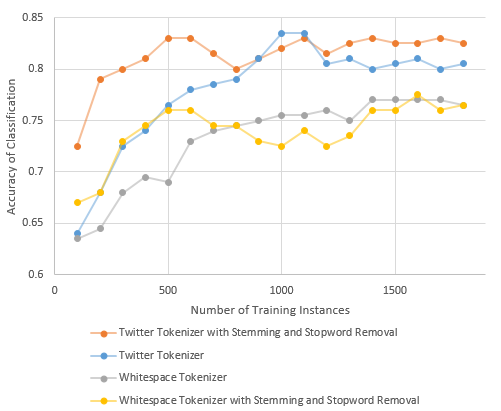
\includegraphics[width=\linewidth]{chart_twitterVSwhitespace}
\caption{Accuracy With Stemming and Stopword Removal}
\label{fig:chart_twitterwhitespace}
\end{figure}

\begin{figure}[ht]
\centering
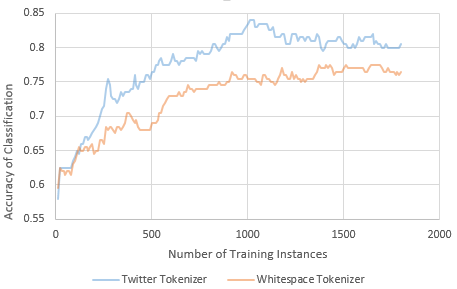
\includegraphics[width=\linewidth]{chart_twitterVSwhitespace_detailed}
\caption{Accuracy For Twitter and Whitespace Tokenizers}
\label{fig:chart_twitterwhitespace_detailed}
\end{figure}


\section{Contributions and Future Work}
We have presented a pipeline for processing tweets that increases accuracy and precision of the resulting models. We introduce a layered approach to tokenization that sees improvements over other rule-based methods. We have built several reusable Java components that extend the Mallet API for processing of data from Twitter. We created a TweetJsonIterator that accepts a file of Twitter's JSON-formatted tweets and creates training Instances containing their values for easy processing during model training. We have implemented several Pipes that can be reused or easily modified to suit a similar Twitter processing purpose. These include Link2Title, Stemmer, SpellCheck, and Tokenize, the latter of which serves as a more extensible tokenizer than Mallet's default. We release our testing utility as a new way of comparing multiple similar pipelines. All code is available through our project website. We also provide a corpus of 100,000 tweets selected by Apple-related keyword and our labeled data set of 2000 tweets. The bash scripts used to filter the data for near-duplicates and spam are also available for download.\\

We could test the robustness of this system by applying this process to other companies for a similar-length time slice of training data. We could also test this model against tweets from a different time span to determine whether the data is subject to temporal overfitting, and to what degree.\\

Yerva et al demonstrate a system of using background knowledge and relatedness, in which current information in the Twitter stream is used to more accurately estimate the priors for a Naive Bayes classification (\citeauthor{journals/ijcsa/YervaMA12}). We believe that inclusion of this in our method could allow us to perform more accurate disambiguation.\\

Wang et al have shown improvements over the bag-of-words approach to text classification using Wikipedia as a thesaurus for term disambiguation. We could use this to enrich the feature set found in tweets and relate similar or co-occurring words in tweets (\citeauthor{Wang:2008:UWC:1510528.1511383}, \citeauthor{Wang:2009:UWK:1554488.1554492}).\\

Our tokenization process makes several simplifying assumptions that we could address. We assume certain classes of emoticons are not used often enough to be significant, and leave punctuation out of our feature set. We could measure the presence of these (and more) features on Twitter data and adjust our tokenization process to reflect that.\\

Sriram et al found that utilizing author profiles provide a good method for further disambiguation of tweets into categories, as authors tend to tweet messages within a limited set of categories. They also delineate a set of eight features (8F) used for training, instead of using the Bag-of-Words approach as we do. Through further analysis of the most useful features found in our approach, we could also choose a discrete set of binary or n-ary features most relevant to this classification task and explore its accuracy versus Bag-of-Words (\citeauthor{Sriram:2010:STC:1835449.1835643}).

\section{ Acknowledgments}
Thank you to Dr. Jin Tian and our class teaching assistant, Ru He, for their helpful guidance during this research project. We also extend our thanks to our friends for their help in manual labeling of tweets.


\bibliographystyle{plainnat}
\bibliography{paper}

%[1] J. Bollen, H. Mao, and X.-J. Zeng. Twitter mood predicts the stock market. Journal of Computational Science, abs/1010.3003, 2010\\

\end{document}
